\chapter{Airport location and characterization}
	\section{Location}
\paragraph{} The main influence on the airport location is the presence of other airports in the area. Since
Jakarta has already one airport, the 18th worldwide, the location has to be selected carefully.
Other factors that influenced the airports final location were the ease to provide the airport
with good connections to the city and a wide area available in order to increase the airports
infrastructure if needed in the future.
After considering all those factors, the location decided can be defined by the following coordinates:

- Latitude: 6°08'21''

- Longitude: 107°06'40''

- Altitude: 30meters approximately.

Since the area chosen is extremely marshy, the excavations to deeper levels are going to be
avoided as much as possible due to its difficulties and cost. However, that type of terrain gives
us some advantage due to its flatness.
	\section{Meteorology}
		\subsection{Temperature}
		\paragraph{}The reference temperature of airports is important to be calculated as soon as possible since it has an effect on the performance of the airplanes during the phases of landing and takeoff. 
		
		In order to calculate this temperature, the definition given by the ICAO will be used. ICAO states that: “The aerodrome reference temperature shall be the monthly mean of the daily maximum temperatures for the hottest month of the year (the hottest month being that which has the highest monthly mean temperature). This temperature shall be averaged over a period of years”.
		
		Taking into account the hypothesis that the temperatures obtained on Soekarno-Hatta Airport can also be used in order to calculate our reference temperature due to the fact that both airports are only separated by a distance of 60km, a comparison study has been made. 
		
		The final reference temperature obtained is \(T_{ref}= 32,38\degree C\). 
		
		The temperature values and study is further detailed in the attachments.
		
		\subsection{Wind}
		\paragraph{}In order to calculate the influence of the winds the first thing done is the graph of the winds intensity and their direction. This graph is commonly called wind rose graph. The graph obtained making use of Microsoft Excel software is:
		
		\begin{figure}[H]
			\centering
			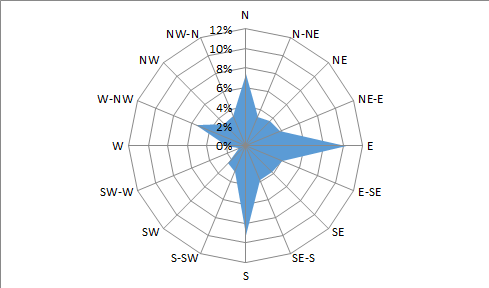
\includegraphics[clip, trim=0.03cm 0cm 0cm 0.03cm, width=1\textwidth]{./images/WIND/ROSE}
			\caption{Wind Rose Graph} %nom de la figura
			\label{} %per denotar una referencia
		\end{figure}
		
		\paragraph{}Once this step is done, the next thing to do is to calculate the coefficient of use by a diagram of
		frequencies. Following the recommendations given by the ICAO on the attachment 14, the maximum value that the transversal component can achieve is 37km/h or 20knots for a runway of >1500m.
		
		The diagram of frequencies basically creates a rectangular area that depends on the runway
		axis, the width of the runway and the maximum transversal component.
		
		After calculating the coefficient of use by all the directions, the graph obtained is the following:

		\begin{figure}[H]
			\centering
			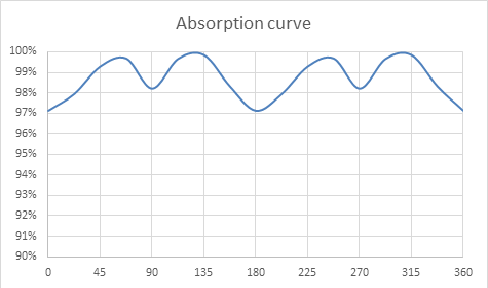
\includegraphics[clip, trim=0cm 0cm 0cm 0cm, width=1\textwidth]{./images/WIND/GRAPH}
			\caption{Coefficient of use depending on the orientation} %nom de la figura
			\label{} %per denotar una referencia
		\end{figure}
		
		\paragraph{}As it can be see, the coefficient is higher than 95\% in any direction. According to that, the final
		orientation chosen is SE-NW.